\documentclass[11pt,a4paper]{article}

\usepackage[utf8]{inputenc}
\usepackage[T1]{fontenc}
\usepackage[english]{babel}
\usepackage{amsmath,amssymb}
\usepackage[top=1.2cm,bottom=1.5cm,left=2cm,right=2cm]{geometry}
\usepackage{graphicx}
\usepackage{booktabs}
\usepackage{hyperref}
\hypersetup{colorlinks=true,linkcolor=black,citecolor=blue,urlcolor=blue}

\title{Question D.3 --- Stratification by Amplitude and the Aggregation Artefact}
\author{}
\date{}

\begin{document}
\maketitle

\noindent Kendall's $\tau_b$ throughout, censored runs imputed to the last rank (Q~D.2).
Confidence intervals are bootstrap intervals over the seeds of the stratum, $2\,000$
resamples, quantiles $2.5\%$ and $97.5\%$. All $120$ coefficients and their intervals are
in \texttt{QCD\_correlations\_stratifiees\_full.parquet} and plotted in
Fig.~\ref{fig:heatmap}; the tables below summarise them.

\section{Why Stratify, and What Pooling Does}

$\Delta e$ drives both sides of every correlation of interest: it shortens
$\tau_{\mathrm{ARF}}$ and raises the evidence available to the detector. A coefficient
computed on the pooled $2\,000$ runs therefore measures that common dependence rather than
any association at a fixed operating point. Each stratum holds $100$ seeds with the
amplitude constant by construction.

\begin{table}[htbp]
  \centering
  \begin{tabular}{lccccc}
    \toprule
    Comparator & pooled & median & range over the 18 & discernible & median CI width \\
    \midrule
    $\tau_{\mathrm{swap}}(10\%)$ & $+1.0000$ & $+1.0000$ & $+1.0000$ to $+1.0000$ & 18/18\rlap{$^{*}$} & $0.000$ \\
    $\tau_{\mathrm{swap}}(25\%)$ & $+0.6446$ & $+0.4932$ & $+0.2616$ to $+0.5484$ & 18/18 & $0.237$ \\
    $\tau_{\mathrm{swap}}(50\%)$ & $+0.5565$ & $+0.3365$ & $+0.0900$ to $+0.3825$ & 15/18 & $0.249$ \\
    $\tau_{\mathrm{swap}}(75\%)$ & $+0.4618$ & $+0.0979$ & $+0.0233$ to $+0.2347$ & 3/18 & $0.266$ \\
    $A(H)$                       & $+0.3965$ & $+0.0526$ & $-0.1009$ to $+0.1212$ & \textbf{0/18} & $0.268$ \\
    $S_{\max}(H)$                & $+0.3147$ & $+0.2129$ & $-0.0470$ to $+0.2954$ & \textbf{15/18} & $0.273$ \\
    \bottomrule
  \end{tabular}
  \caption{Pooled against stratified $\tau_b(\tau_{\mathrm{ARF}}, \cdot)$ on the 18
  amplitudes of the decision domain. ``Discernible'' counts the cells whose bootstrap
  interval excludes zero, the rule fixed in Q~D.4. $^{*}$tautological, see below.}
  \label{tab:agregation}
\end{table}

For $A(H)$ the pooled coefficient is $+0.3965$ against a stratified median of $+0.0526$, a
factor of $7.5$, and the stratified value is indistinguishable from zero under this
protocol at every one of the 18 amplitudes. The pooled coefficient manufactures a link
rather than confirming a weak one: it is Simpson's paradox on $\Delta e$, since within each
stratum there is nothing while across strata both quantities move with the amplitude. The
effect is strongest exactly where the within-stratum association is weakest, ratio $7.54$
for $A(H)$ and $4.72$ for $\tau_{\mathrm{swap}}(75\%)$ against only $1.48$ for
$S_{\max}(H)$, which does carry a genuine signal. No pooled coefficient is quoted as a
result anywhere in this work.

\paragraph{The tautological row.} At $M = 10$ a quota of $10\%$ requires one tree, so
$\tau_{\mathrm{swap}}(10\%) = \tau_{\mathrm{ARF}}$ by definition (Q~C.1a) and its $\tau_b$
is $1.000000$ at all $20$ amplitudes with interval $[1.000 ; 1.000]$, by identity rather
than performance. The row is kept and hatched in Fig.~\ref{fig:heatmap} rather than
deleted, so a reader can check that the instrumentation reproduces an identity it should;
it carries no other evidence. The precedent is $S_{\max}(H)$ under test B2, whose AUC of
$1.000$ is tautological in the same sense. Relatedly, at $M = 10$ neither $q = 25\%$ nor
$q = 75\%$ is exactly attainable ($3$ trees, so $30\%$; $8$ trees, so $80\%$); the labels
follow Q~C.1 but name the attainable quota above the nominal one.

\begin{figure}[htbp]
  \centering
  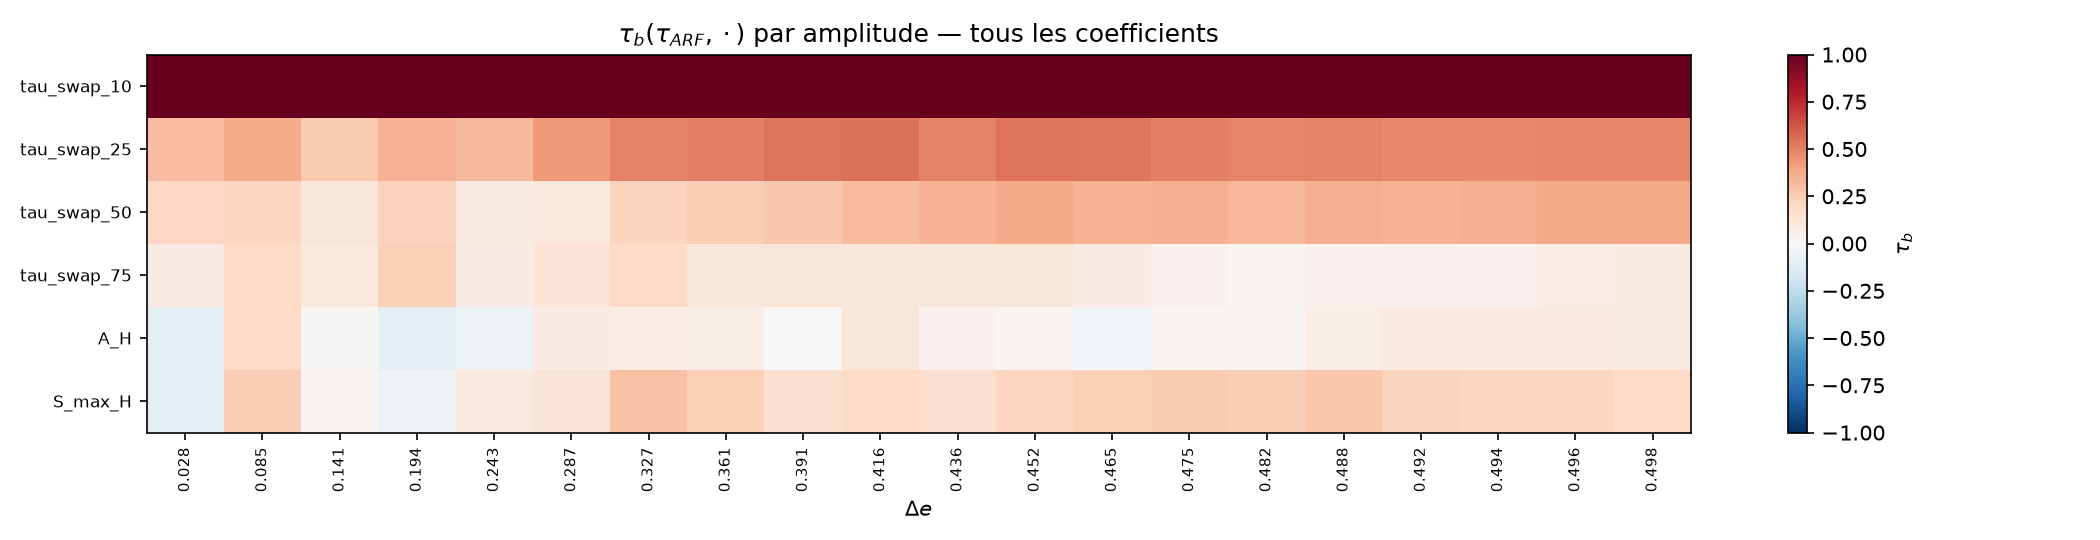
\includegraphics[width=\textwidth]{resultats_R2/resultats/figures/Fig_QD_heatmap_taub_full.png}
  \caption{$\tau_b(\tau_{\mathrm{ARF}}, \cdot)$ for every comparator at every amplitude.
  All $120$ coefficients published, no post hoc selection. Hatched row: tautological.}
  \label{fig:heatmap}
\end{figure}

\section{The Central Result of Q~D}

The two quantities at the bottom of Table~\ref{tab:agregation} play different roles, and
conflating them changes the answer. $A(H)$ is the accumulated excess error over the
horizon; $S_{\max}(H)$ is the maximum of the CUSUM path, and \emph{it is $S_{\max}(H)$ that
decides the alarm}, since the alarm is by definition the crossing of $\lambda$ by
$S_{\max}$. A claim that $\tau_{\mathrm{ARF}}$ carries no information about the evidence
offered to the detector is attached to the wrong object if it rests on $A(H)$ alone.

\begin{quote}
$\tau_{\mathrm{ARF}}$ carries \textbf{no information} about $A(H)$: median $+0.0526$, every
interval straddling zero, 0 of 18 amplitudes. It carries a \textbf{weak but real}
association with $S_{\max}(H)$: median $+0.2129$, discernible at 15 of 18, which is every
amplitude from $\Delta e = 0.287$ upwards without exception. Below $\Delta e = 0.287$ it is
not distinguishable from zero either.
\end{quote}

The strongest cells are $+0.2954$ $[+0.1832 ; +0.4063]$ at $\Delta e = 0.327$ and $+0.2764$
$[+0.1478 ; +0.4055]$ at $\Delta e = 0.488$; the boundary cell is $+0.1308$
$[+0.0027 ; +0.2519]$ at $\Delta e = 0.287$. Read with Q~D.2, the residual bias reinforces
this reading: $A(H)$ and $S_{\max}(H)$ are never censored and carry no tie blocks, so the
correction applies on the $\tau_{\mathrm{ARF}}$ side only and displaces both coefficients
towards zero. The $A(H)$ null is not an artefact of ties inflating it, and the
$S_{\max}(H)$ signal is if anything understated.

\paragraph{Reservations.} The decision domain holds $108$ cells, of which $68$ are
significant at $5\%$ with no multiplicity correction; the $S_{\max}(H)$ signal above
$\Delta e = 0.287$ runs to 15 consecutive amplitudes in the same direction and is far too
systematic to be a multiplicity artefact, but individual cells near the detectability
threshold are not quoted alone. That threshold is $0.13295637$, quoted exactly since a
rounded value would not reproduce the \texttt{discernable} column, which Q~D.4 discusses
and does not adopt. Everything here is measured at $M = 10$ on one campaign, and the two
amplitudes below $\Delta e = 0.10$ are outside the decision domain, excluded from the
medians though present in Fig.~\ref{fig:heatmap}.

\end{document}
